\documentclass[11pt]{article}
%\parskip 1.0\parskip plus 3pt minus 1pt
\renewcommand{\baselinestretch}{1.5}

\setlength{\oddsidemargin}{-0.1in}
\setlength{\evensidemargin}{-0.1in} 
\setlength{\textwidth}{6.54in}
\setlength{\topmargin}{0in} 
\setlength{\textheight}{8.5in}
%\setlength{\oddsidemargin}{0in}
%\setlength{\evensidemargin}{0.15in} 
%\setlength{\textwidth}{6.2in}
%\setlength{\topmargin}{-0.3in} 
%\setlength{\textheight}{8.9in}

\linespread{1}

\usepackage{makeidx}
\usepackage{amsmath,amssymb, amsthm}
\usepackage{latexsym,remreset}
\usepackage[toc,page]{appendix}
\usepackage{graphicx}
\usepackage{multirow}
\usepackage{bbm}
%\usepackage[pdftex]{graphicx} 

\usepackage{url}
%% Define a new 'leo' style for the package that will use a smaller font.
\makeatletter
\def\url@leostyle{%
  \@ifundefined{selectfont}{\def\UrlFont{\sf}}{\def\UrlFont{\small\ttfamily}}}
\makeatother
%% Now actually use the newly defined style.
\urlstyle{leo}

\newtheorem{assumption}{Assumption}
\newtheorem{definition}{Definition}
\newtheorem{lemma}{Lemma}
\newtheorem{proposition}{Proposition}
\newtheorem{corollary}{Corollary}
\newtheorem{remark}{Remark}
\newtheorem{theorem}{Theorem}
\newcommand{\mb}[1]{\ensuremath{\boldsymbol{#1}}}
\newcommand{\vol}{{\sf volume}}
\newcommand{\Stochb}{$\Pi_{\mathrm {Stoch}}(b)$}
\newcommand{\tf}{\text{translation factor}}

\title{ISyE6669 Homework 8\\
Fall 2025}
\author{}
\date{}

\begin{document}
\maketitle



	\begin{enumerate}
		\item Consider the following linear program:
	\begin{eqnarray*}
		&\begin{array}{cccccc}
			\min & -x_1 & - & 2x_2 &  & \\
			\text{s.t.} & x_1  & - & x_2  & \leq & 1 \\
			& 2x_1 & - & x_2 & \geq & -1 \\
			& 2x_1 & + & x_2 & \leq & 5 \\
		\end{array} \\
		&\begin{array}{rr}
			x_1\geq 0, & x_2\geq 0. \\
		\end{array}
	\end{eqnarray*}
		Graph the constraints of this linear program, and indicate the feasible region.
		
		\textbf{Solution:}
		Please refer to the accompanying figure for the graphical representation of the constraints and feasible region.
		
		\begin{figure}[h]
		\centering
		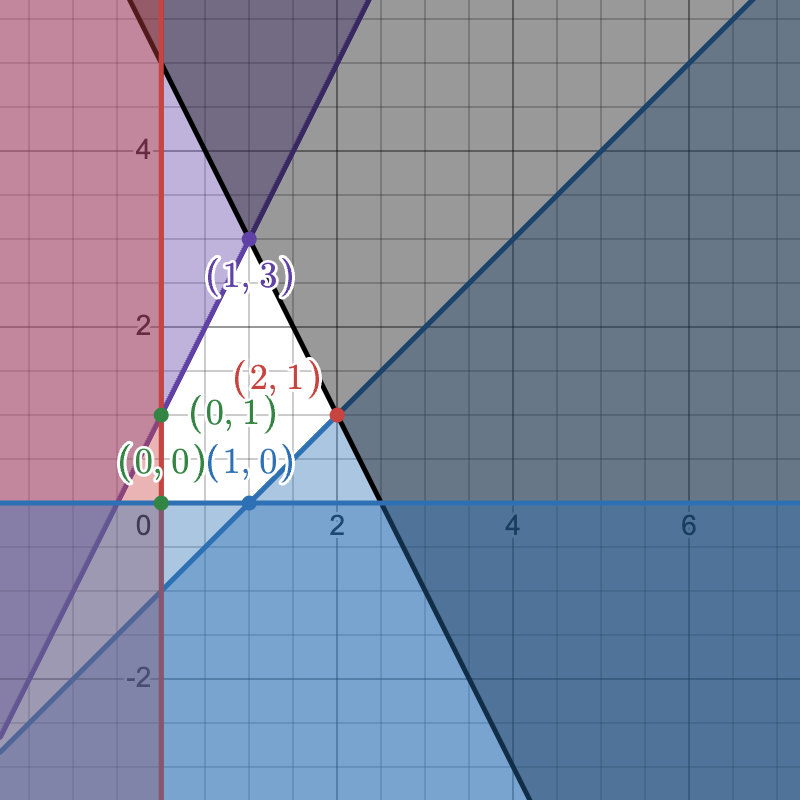
\includegraphics[width=0.7\textwidth]{HW7-3a.png}
		\caption{Linear program constraints and feasible region}
		\end{figure}
		
	\item To solve this problem using the simplex method, first transform it into a standard form LP.

Let $x_3$, $x_4$, $x_5$ be the slack variables with respect to the first, second, third constraint respectively. Denote $\mb{x}=[x_1,x_2,x_3,x_4,x_5]^\top$ as the vector of variables, and use the standard form notation: 
\begin{align*}
\min \quad & \mb{c}^\top\mb{x} \\
\text{s.t.}\quad & \mb{A}\mb{x} = \mb{b} \\
& \mb{x}\geq \mb{0},
\end{align*}
specify $\mb{c},\mb{A},\mb{b}$ for the above problem.

\textbf{Solution:}
We introduce slack variables $x_3, x_4, x_5$ to convert inequalities to equalities. The standard form LP becomes:
\begin{align*}
\min \quad & -x_1 - 2x_2 \\
\text{s.t.}\quad & x_1 - x_2 + x_3 = 1 \\
& -2x_1 + x_2 + x_4 = 1 \\
& 2x_1 + x_2 + x_5 = 5 \\
& x_1, x_2, x_3, x_4, x_5 \geq 0
\end{align*}

Therefore, we have:
\begin{align*}
\mb{c} &= \begin{bmatrix} -1 \\ -2 \\ 0 \\ 0 \\ 0 \end{bmatrix}, \quad
\mb{A} = \begin{bmatrix} 
1 & -1 & 1 & 0 & 0 \\
-2 & 1 & 0 & 1 & 0 \\
2 & 1 & 0 & 0 & 1
\end{bmatrix}, \quad
\mb{b} = \begin{bmatrix} 1 \\ 1 \\ 5 \end{bmatrix}
\end{align*} 

\item Now we want to solve the above standard-form linear program by the simplex method. If in an iteration of the Simplex method, there is any ambiguity about which nonbasic variable to enter the basis or which basic variable to exit the basis, use Bland's rule. 


\begin{enumerate}
	
	\item For each iteration of the simplex method, write down the following information in the format given below:
	\begin{itemize}
		\item Iteration $k=\underline{\text{numerical value, e.g. 1, 2, ...}}$;
		\item Basis $\mb{B} = [\mb{A}_i,\mb{A}_j,\mb{A}_k]=\underline{\text{numerical value}}$ (i.e. you need to specify $i,j,k$ as well as the numerical values of the columns);
		\item Basis inverse $\mb{B}^{-1} = \underline{\text{numerical value}}$;
		\item Basic variable $\mb{x}_B = [x_i, x_j, x_k] = \underline{\text{numerical value}}$ (you need to specify $i,j,k$ and numerical values of $x_i,x_j,x_k$);
		\item Nonbasic variable $\mb{x}_N = [x_p, x_q] = \underline{\text{numerical value}}$ (you need to specify $p,q$ and numerical values of $x_p,x_q$);
		\item Reduced cost for each nonbasic variable $\bar{c}_p = c_p - \mb{c}_B^\top\mb{B}^{-1}\mb{A}_? = \underline{\text{numerical values}}$; Same for $\bar{c}_q$; (you need to determine the index ``?'' for $\mb{A}_?$);
		\item Is the current solution optimal? If not, which nonbasic variable enters the basis?
		\item Direction $\mb{d}_B = -\mb{B}^{-1}\mb{A}_?=\underline{\text{numerical value}}$. Does the simplex method terminate with an unbounded optimum?
		\item Min-ratio test $\theta^* = \min_{i : {d}_{B(i)<0}}\{x_{B(i)}/(-d_{B(i)})\}=\min\{\underline{\text{numerical values of the ratios}}\}=\underline{\text{numerical value of $\theta^*$}}$. 
		\item Which basic variable exits the basis?
	\end{itemize}
	Start at iteration $k=1$ with the basis $\mb{B}^1=[\mb{A}_3,\mb{A}_4,\mb{A}_5]$. Solve the above linear program with simplex method and write down all the information required above for each iteration. Also indicate the basic feasible solution at each step on the picture in $(x_1, x_2)$. What is the optimal solution of the above LP in $(x_1, \dots, x_5)$? What is the optimal cost?
\end{enumerate}
From this exercise, you can see how the simplex method works and geometrically what each step is doing. 

\textbf{Solution:}

\textbf{General Framework for Simplex Method:}

Let us first establish the general mathematical framework. For a standard form LP with basis matrix $\mb{B}$ and nonbasic matrix $\mb{N}$, we have:
\begin{align}
\mb{A}\mb{x} = \mb{B}\mb{x}_B + \mb{N}\mb{x}_N = \mb{b} \tag{1}
\end{align}

Multiplying by $\mb{B}^{-1}$ from the left:
\begin{align}
\mb{x}_B = \mb{B}^{-1}\mb{b} - \mb{B}^{-1}\mb{N}\mb{x}_N \tag{2}
\end{align}

The objective function can be written as:
\begin{align}
Z &= \mb{c}_B^\top\mb{x}_B + \mb{c}_N^\top\mb{x}_N \tag{3}
\end{align}

Substituting equation (2) into (3):
\begin{align}
Z &= \mb{c}_B^\top(\mb{B}^{-1}\mb{b} - \mb{B}^{-1}\mb{N}\mb{x}_N) + \mb{c}_N^\top\mb{x}_N \nonumber \\
&= \mb{c}_B^\top\mb{B}^{-1}\mb{b} + (\mb{c}_N^\top - \mb{c}_B^\top\mb{B}^{-1}\mb{N})\mb{x}_N \tag{4}
\end{align}

The reduced costs for nonbasic variables are:
\begin{align}
\bar{\mb{c}}_N = \mb{c}_N^\top - \mb{c}_B^\top\mb{B}^{-1}\mb{N} \tag{5}
\end{align}

For entering variable selection, we choose the nonbasic variable with the most negative reduced cost (Bland's rule for tie-breaking). The direction vector is:
\begin{align}
\mb{d}_B = -\mb{B}^{-1}\mb{A}_j \tag{6}
\end{align}
where $\mb{A}_j$ is the column corresponding to the entering variable.

\textbf{Iteration $k=1$:}

\begin{figure}[h]
\centering
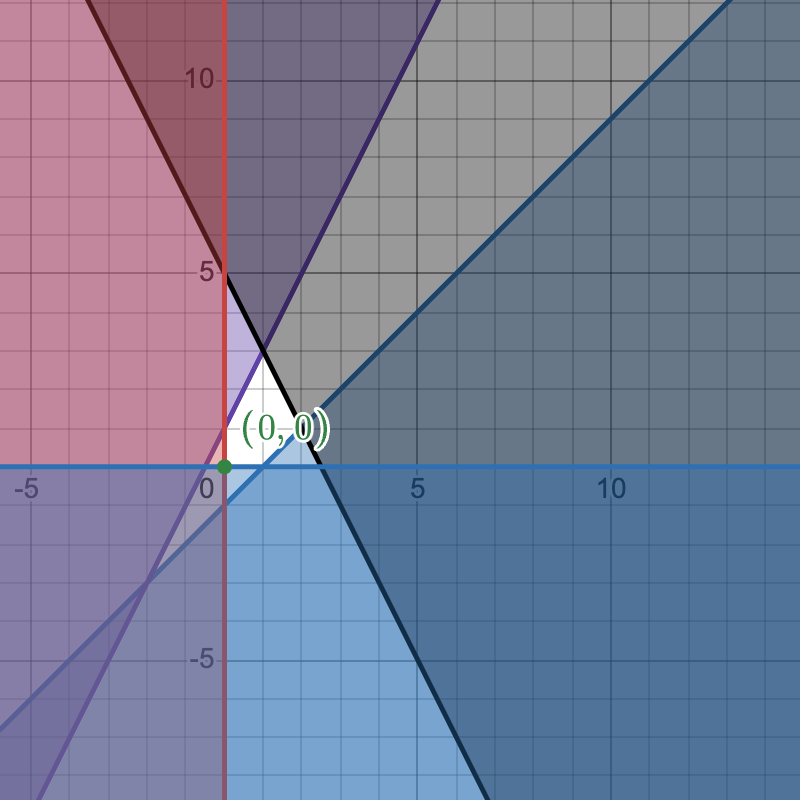
\includegraphics[width=0.5\textwidth]{HW8-3-1.png}
\caption{Iteration 1: Basic feasible solution $(x_1, x_2) = (0, 0)$}
\end{figure}

\begin{itemize}
\item Iteration $k=1$;

\item Basis $\mb{B}^1 = [\mb{A}_3,\mb{A}_4,\mb{A}_5] = \begin{bmatrix} 1 & 0 & 0 \\ 0 & 1 & 0 \\ 0 & 0 & 1 \end{bmatrix}$;

\item Basis inverse $\mb{B}^{-1} = \begin{bmatrix} 1 & 0 & 0 \\ 0 & 1 & 0 \\ 0 & 0 & 1 \end{bmatrix}$;

\item Basic variables $\mb{x}_B = [x_3, x_4, x_5] = \mb{B}^{-1}\mb{b} = \begin{bmatrix} 1 \\ 1 \\ 5 \end{bmatrix}$;

\item Nonbasic variables $\mb{x}_N = [x_1, x_2] = \begin{bmatrix} 0 \\ 0 \end{bmatrix}$;

\item For nonbasic variables, we have $\mb{c}_B = \begin{bmatrix} 0 \\ 0 \\ 0 \end{bmatrix}$, $\mb{c}_N = \begin{bmatrix} -1 \\ -2 \end{bmatrix}$, and $\mb{N} = \begin{bmatrix} 1 & -1 \\ -2 & 1 \\ 2 & 1 \end{bmatrix}$.

Using equation (5), the reduced costs are:
\begin{align*}
\bar{c}_1 &= c_1 - \mb{c}_B^\top\mb{B}^{-1}\mb{A}_1 = -1 - \begin{bmatrix} 0 & 0 & 0 \end{bmatrix} \begin{bmatrix} 1 \\ -2 \\ 2 \end{bmatrix} = -1 \\
\bar{c}_2 &= c_2 - \mb{c}_B^\top\mb{B}^{-1}\mb{A}_2 = -2 - \begin{bmatrix} 0 & 0 & 0 \end{bmatrix} \begin{bmatrix} -1 \\ 1 \\ 1 \end{bmatrix} = -2
\end{align*}

\item Objective function value using equation (4):
\begin{align*}
Z = \mb{c}_B^\top\mb{B}^{-1}\mb{b} + \bar{\mb{c}}_N^\top\mb{x}_N = \begin{bmatrix} 0 & 0 & 0 \end{bmatrix} \begin{bmatrix} 1 \\ 1 \\ 5 \end{bmatrix} + \begin{bmatrix} -1 & -2 \end{bmatrix} \begin{bmatrix} 0 \\ 0 \end{bmatrix} = 0
\end{align*}

\item The current solution is not optimal since both $\bar{c}_1 = -1 < 0$ and $\bar{c}_2 = -2 < 0$. By Bland's rule, we choose the variable with the smallest subscript among negative reduced costs. Since both are negative, we choose $x_1$ to enter the basis.

\item Direction using equation (6): $\mb{d}_B = -\mb{B}^{-1}\mb{A}_1 = -\begin{bmatrix} 1 & 0 & 0 \\ 0 & 1 & 0 \\ 0 & 0 & 1 \end{bmatrix} \begin{bmatrix} 1 \\ -2 \\ 2 \end{bmatrix} = \begin{bmatrix} -1 \\ 2 \\ -2 \end{bmatrix}$. 

Since $d_{B(2)} = 2 > 0$ and $d_{B(3)} = -2 < 0$, the method does not terminate with unbounded optimum.

\item Min-ratio test: $\theta^* = \min_{i : d_{B(i)} < 0}\{x_{B(i)}/(-d_{B(i)})\} = \min\{x_3/(-d_{B(1)}), x_5/(-d_{B(3)})\} = \min\{1/1, 5/2\} = \min\{1, 2.5\} = 1$.

\item The basic variable $x_3$ exits the basis (smallest ratio).
\end{itemize}

\textbf{Iteration $k=2$:}

\begin{figure}[h]
\centering
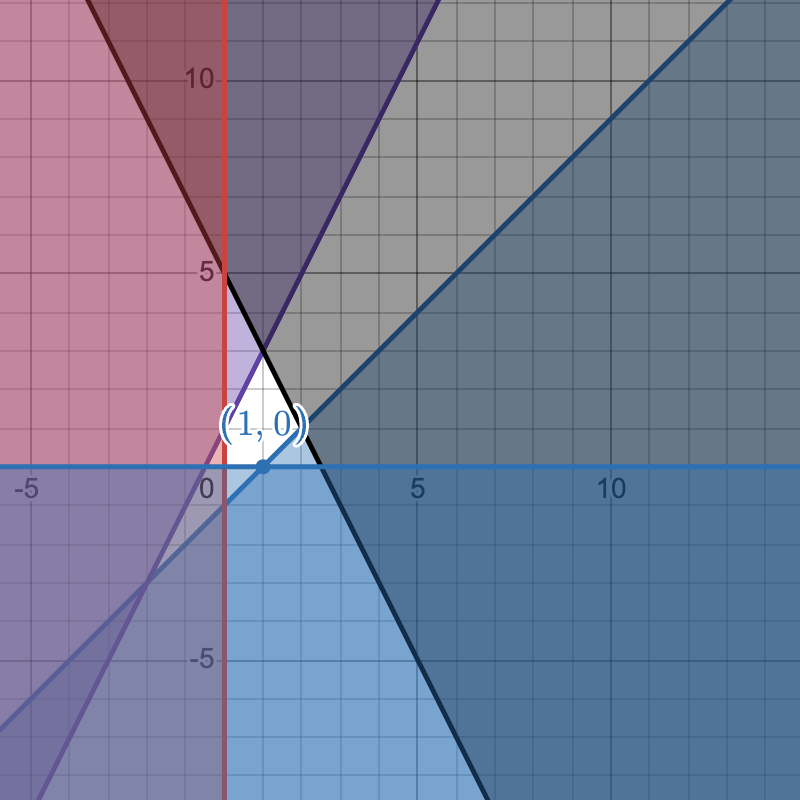
\includegraphics[width=0.5\textwidth]{HW8-3-2.png}
\caption{Iteration 2: Basic feasible solution $(x_1, x_2) = (1, 0)$}
\end{figure}

\begin{itemize}
\item Iteration $k=2$;

\item Basis $\mb{B}^2 = [\mb{A}_1,\mb{A}_4,\mb{A}_5] = \begin{bmatrix} 1 & 0 & 0 \\ -2 & 1 & 0 \\ 2 & 0 & 1 \end{bmatrix}$;

\item Basis inverse $\mb{B}^{-1} = \begin{bmatrix} 1 & 0 & 0 \\ 2 & 1 & 0 \\ -2 & 0 & 1 \end{bmatrix}$;

\item Basic variables $\mb{x}_B = [x_1, x_4, x_5] = \mb{B}^{-1}\mb{b} = \begin{bmatrix} 1 & 0 & 0 \\ 2 & 1 & 0 \\ -2 & 0 & 1 \end{bmatrix} \begin{bmatrix} 1 \\ 1 \\ 5 \end{bmatrix} = \begin{bmatrix} 1 \\ 3 \\ 3 \end{bmatrix}$;

\item Nonbasic variables $\mb{x}_N = [x_2, x_3] = \begin{bmatrix} 0 \\ 0 \end{bmatrix}$;

\item For this iteration, $\mb{c}_B = \begin{bmatrix} -1 \\ 0 \\ 0 \end{bmatrix}$, $\mb{c}_N = \begin{bmatrix} -2 \\ 0 \end{bmatrix}$, and $\mb{N} = \begin{bmatrix} -1 & 1 \\ 1 & 0 \\ 1 & 0 \end{bmatrix}$.

Using equation (5):
\begin{align*}
\bar{c}_2 &= c_2 - \mb{c}_B^\top\mb{B}^{-1}\mb{A}_2 = -2 - \begin{bmatrix} -1 & 0 & 0 \end{bmatrix} \begin{bmatrix} 1 & 0 & 0 \\ 2 & 1 & 0 \\ -2 & 0 & 1 \end{bmatrix} \begin{bmatrix} -1 \\ 1 \\ 1 \end{bmatrix} = -2 - (-1)(1) = -3 \\
\bar{c}_3 &= c_3 - \mb{c}_B^\top\mb{B}^{-1}\mb{A}_3 = 0 - \begin{bmatrix} -1 & 0 & 0 \end{bmatrix} \begin{bmatrix} 1 & 0 & 0 \\ 2 & 1 & 0 \\ -2 & 0 & 1 \end{bmatrix} \begin{bmatrix} 1 \\ 0 \\ 0 \end{bmatrix} = 0 - (-1)(1) = 1
\end{align*}

\item Objective function value:
\begin{align*}
Z = \mb{c}_B^\top\mb{B}^{-1}\mb{b} = \begin{bmatrix} -1 & 0 & 0 \end{bmatrix} \begin{bmatrix} 1 \\ 3 \\ 3 \end{bmatrix} = -1
\end{align*}

\item Since $\bar{c}_2 = -3 < 0$, the current solution is not optimal. $x_2$ enters the basis.

\item Direction: $\mb{d}_B = -\mb{B}^{-1}\mb{A}_2 = -\begin{bmatrix} 1 & 0 & 0 \\ 2 & 1 & 0 \\ -2 & 0 & 1 \end{bmatrix} \begin{bmatrix} -1 \\ 1 \\ 1 \end{bmatrix} = \begin{bmatrix} 1 \\ -3 \\ 1 \end{bmatrix}$.

Since $d_{B(2)} = -3 < 0$, the method does not terminate with unbounded optimum.

\item Min-ratio test: $\theta^* = \min_{i : d_{B(i)} < 0}\{x_{B(i)}/(-d_{B(i)})\} = \min\{x_4/3\} = \min\{3/3\} = 1$.

\item The basic variable $x_4$ exits the basis.
\end{itemize}

\textbf{Iteration $k=3$:}
\begin{itemize}
\item Iteration $k=3$;

\item Basis $\mb{B}^3 = [\mb{A}_1,\mb{A}_2,\mb{A}_5] = \begin{bmatrix} 1 & -1 & 0 \\ -2 & 1 & 0 \\ 2 & 1 & 1 \end{bmatrix}$;

\item Basis inverse $\mb{B}^{-1} = \begin{bmatrix} 1 & 1 & 0 \\ 2 & 1 & 0 \\ -4 & -3 & 1 \end{bmatrix}$;

\item The basic variable $x_5$ exits the basis.
\end{itemize}

\textbf{Iteration $k=3$:}

\begin{figure}[h]
\centering
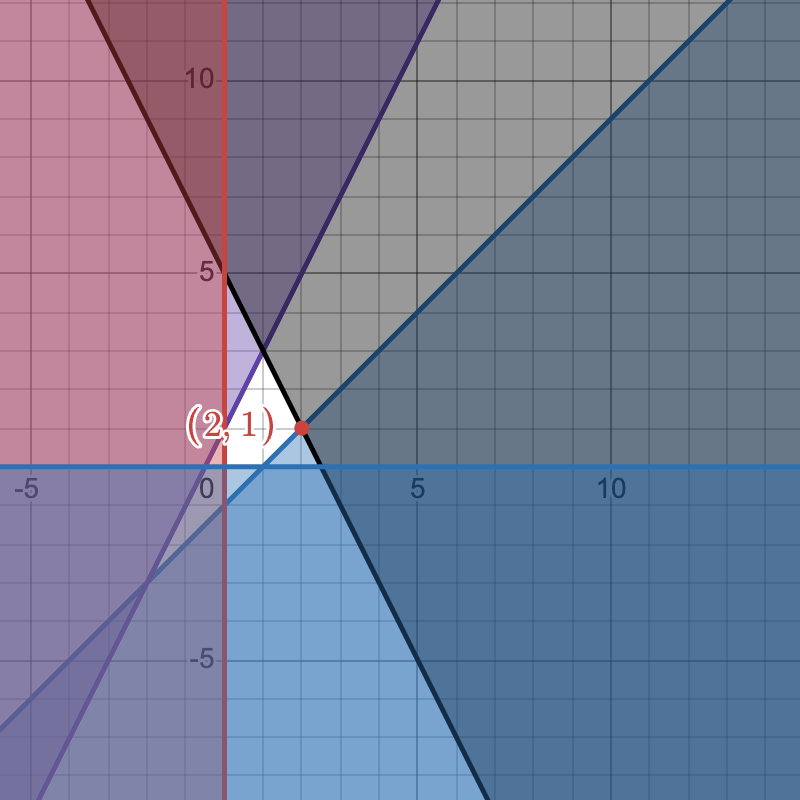
\includegraphics[width=0.5\textwidth]{HW8-3-3.png}
\caption{Iteration 3: Basic feasible solution $(x_1, x_2) = (2, 1)$}
\end{figure}

\begin{itemize}
\item Iteration $k=3$;

\item Basis $\mb{B}^3 = [\mb{A}_1,\mb{A}_2,\mb{A}_4] = \begin{bmatrix} 1 & -1 & 0 \\ -2 & 1 & 1 \\ 2 & 1 & 0 \end{bmatrix}$;

\item Basis inverse $\mb{B}^{-1} = \begin{bmatrix} 1/3 & 0 & 1/3 \\ -2/3 & 0 & 1/3 \\ 4/3 & 1 & 1/3 \end{bmatrix}$;

\item Basic variables $\mb{x}_B = [x_1, x_2, x_4] = \mb{B}^{-1}\mb{b} = \begin{bmatrix} 2 \\ 1 \\ 4 \end{bmatrix}$;

\item Nonbasic variables $\mb{x}_N = [x_3, x_5] = \begin{bmatrix} 0 \\ 0 \end{bmatrix}$;

\item For this iteration, $\mb{c}_B = \begin{bmatrix} -1 \\ -2 \\ 0 \end{bmatrix}$, $\mb{c}_N = \begin{bmatrix} 0 \\ 0 \end{bmatrix}$, and $\mb{N} = \begin{bmatrix} 1 & 0 \\ 0 & 0 \\ 0 & 1 \end{bmatrix}$.

Using equation (5):
\begin{align*}
\bar{c}_3 &= c_3 - \mb{c}_B^\top\mb{B}^{-1}\mb{A}_3 = 0 - \begin{bmatrix} -1 & -2 & 0 \end{bmatrix} \begin{bmatrix} 1/3 & 0 & 1/3 \\ -2/3 & 0 & 1/3 \\ 4/3 & 1 & 1/3 \end{bmatrix} \begin{bmatrix} 1 \\ 0 \\ 0 \end{bmatrix} = -1 \\
\bar{c}_5 &= c_5 - \mb{c}_B^\top\mb{B}^{-1}\mb{A}_5 = 0 - \begin{bmatrix} -1 & -2 & 0 \end{bmatrix} \begin{bmatrix} 1/3 \\ 1/3 \\ 1/3 \end{bmatrix} = 1
\end{align*}

\item Objective function value:
\begin{align*}
Z = \mb{c}_B^\top\mb{B}^{-1}\mb{b} = \begin{bmatrix} -1 & -2 & 0 \end{bmatrix} \begin{bmatrix} 2 \\ 1 \\ 4 \end{bmatrix} = -4
\end{align*}

\item Since $\bar{c}_3 = -1 < 0$, the current solution is not optimal. $x_3$ enters the basis.

\item Direction: $\mb{d}_B = -\mb{B}^{-1}\mb{A}_3 = -\begin{bmatrix} 1/3 & 0 & 1/3 \\ -2/3 & 0 & 1/3 \\ 4/3 & 1 & 1/3 \end{bmatrix} \begin{bmatrix} 1 \\ 0 \\ 0 \end{bmatrix} = \begin{bmatrix} -1/3 \\ 2/3 \\ -4/3 \end{bmatrix}$.

Since $d_{B(1)} = -1/3 < 0$ and $d_{B(3)} = -4/3 < 0$, the method does not terminate with unbounded optimum.

\item Min-ratio test: $\theta^* = \min_{i : d_{B(i)} < 0}\{x_{B(i)}/(-d_{B(i)})\} = \min\{x_1/(1/3), x_4/(4/3)\} = \min\{2 \times 3, 4 \times 3/4\} = \min\{6, 3\} = 3$.

\item The basic variable $x_4$ exits the basis.
\end{itemize}

\textbf{Iteration $k=4$:}

\begin{figure}[h]
\centering
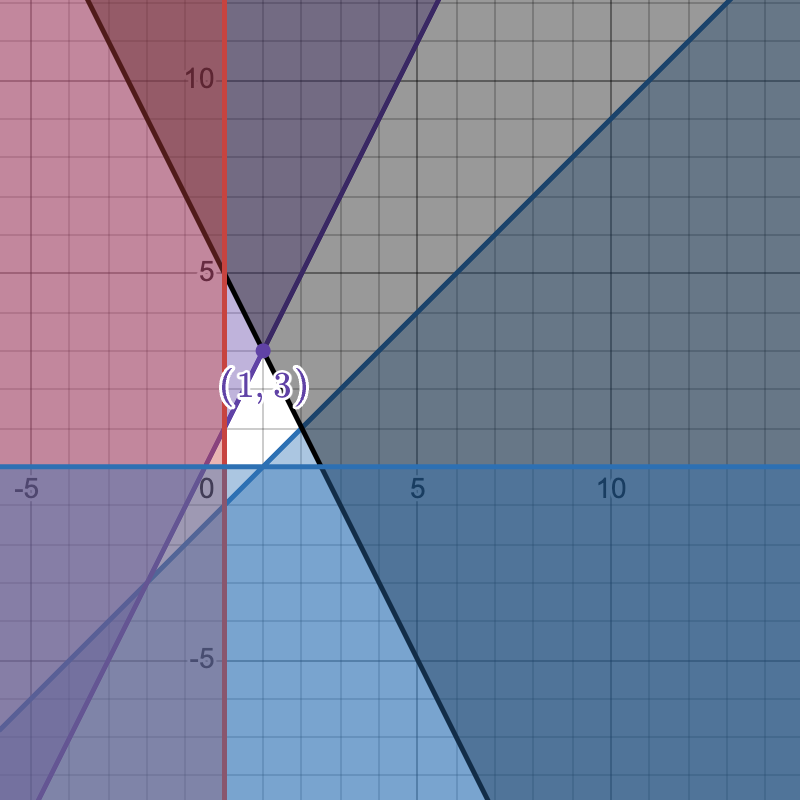
\includegraphics[width=0.5\textwidth]{HW8-3-4.png}
\caption{Iteration 4: Basic feasible solution $(x_1, x_2) = (1, 3)$ - Optimal}
\end{figure}

\begin{itemize}
\item Iteration $k=4$;

\item Basis $\mb{B}^4 = [\mb{A}_1,\mb{A}_2,\mb{A}_3] = \begin{bmatrix} 1 & -1 & 1 \\ -2 & 1 & 0 \\ 2 & 1 & 0 \end{bmatrix}$;

\item Basis inverse $\mb{B}^{-1} = \begin{bmatrix} 0 & -1/4 & 1/4 \\ 0 & 1/2 & 1/2 \\ 1 & 3/4 & 1/4 \end{bmatrix}$;

\item Basic variables $\mb{x}_B = [x_1, x_2, x_3] = \mb{B}^{-1}\mb{b} = \begin{bmatrix} 1 \\ 3 \\ 3 \end{bmatrix}$;

\item Nonbasic variables $\mb{x}_N = [x_4, x_5] = \begin{bmatrix} 0 \\ 0 \end{bmatrix}$;

\item For this iteration, $\mb{c}_B = \begin{bmatrix} -1 \\ -2 \\ 0 \end{bmatrix}$, $\mb{c}_N = \begin{bmatrix} 0 \\ 0 \end{bmatrix}$, and $\mb{N} = \begin{bmatrix} 0 & 0 \\ 1 & 0 \\ 0 & 1 \end{bmatrix}$.

Using equation (5):
\begin{align*}
\bar{c}_4 &= c_4 - \mb{c}_B^\top\mb{B}^{-1}\mb{A}_4 = 0 - \begin{bmatrix} -1 & -2 & 0 \end{bmatrix} \begin{bmatrix} 0 \\ 1/2 \\ 3/4 \end{bmatrix} = 1 \\
\bar{c}_5 &= c_5 - \mb{c}_B^\top\mb{B}^{-1}\mb{A}_5 = 0 - \begin{bmatrix} -1 & -2 & 0 \end{bmatrix} \begin{bmatrix} 1/4 \\ 1/2 \\ 1/4 \end{bmatrix} = 5/4
\end{align*}

\item Objective function value:
\begin{align*}
Z = \mb{c}_B^\top\mb{B}^{-1}\mb{b} = \begin{bmatrix} -1 & -2 & 0 \end{bmatrix} \begin{bmatrix} 1 \\ 3 \\ 3 \end{bmatrix} = -7
\end{align*}

\item Since both reduced costs are non-negative ($\bar{c}_4 = 1 > 0$ and $\bar{c}_5 = 5/4 > 0$), the current solution is optimal.

\end{itemize}

\textbf{Summary:}
The optimal solution is $\mb{x}^* = [1, 3, 3, 0, 0]^\top$ with optimal objective value $Z^* = -7$.

In terms of the original variables $(x_1, x_2)$, the optimal solution is $(x_1^*, x_2^*) = (1, 3)$ with optimal cost $-1 \times 1 - 2 \times 3 = -7$.

The basic feasible solutions visited during the Simplex method correspond to:
\begin{itemize}
\item Iteration 1: $(x_1, x_2) = (0, 0)$ with cost $0$
\item Iteration 2: $(x_1, x_2) = (1, 0)$ with cost $-1$ 
\item Iteration 3: $(x_1, x_2) = (2, 1)$ with cost $-4$
\item Iteration 4: $(x_1, x_2) = (1, 3)$ with cost $-7$ (optimal)
\end{itemize}
\end{enumerate}
\end{document}